%%% PREAMBLE - Do not touch %%%%%%%%%%%%%%%%%%%%%%%%%%%%%%%%%%%%%%%%%%%%%%%%%%%%%%
\documentclass[10pt,twocolumn,letterpaper]{article}
\usepackage[ansinew]{inputenc}
\usepackage[portuges,brazil,english]{babel}
\usepackage{model}
\usepackage{times}
\usepackage{epsfig}
\usepackage{graphicx}
\usepackage{amsmath}
\usepackage{amssymb}
\usepackage{color}
\usepackage{float}
\usepackage[pagebackref=true,breaklinks=true,letterpaper=true,colorlinks,bookmarks=false]{hyperref}

\cvprfinalcopy % *** Uncomment this line for the final submission
\def\httilde{\mbox{\tt\raisebox{-.5ex}{\symbol{126}}}}
\ifcvprfinal\pagestyle{empty}\fi

\newcommand{\TODO}[1]{TODO: #1}
\newcommand{\CITEONE}[2]{\mbox{#1 \cite{#2}}}
\newcommand{\CITETWO}[3]{\mbox{#1 and #2 \cite{#3}}}
\newcommand{\CITEN}[2]{\mbox{#1 et al. \cite{#2}}}

%%% Paper beginning %%%%%%%%%%%%%%%%%%%%%%%%%%%%%%%%%%%%%%%%%%%%%%%%%%%%%%%%%%%%%%
\begin{document}

%%% Title and authors %%%%%%%%%%%%%%%%%%%%%%%%%%%%%%%%%%%%%%%%%%%%%%%%%%%%%%%%%%%%
\title{Assignment 3 - MO444}
\author{Pedro Henrique M. X. Zacarin\thanks{\textbf{Contact}: \tt\small{phzacarin@gmail.com}}\\
}

%%% Abstract %%%%%%%%%%%%%%%%%%%%%%%%%%%%%%%%%%%%%%%%%%%%%%%%%%%%%%%%%%%%%%%%%%%%%
\maketitle
\begin{abstract}
In this assignment, the goal was to clusterize all the headlines from a dataset consisting of 1 million headlines from the Australian Broadcast Corporation (ABC) over a period of 15 years based on topics.
\end{abstract}

%%% Introduction %%%%%%%%%%%%%%%%%%%%%%%%%%%%%%%%%%%%%%%%%%%%%%%%%%%%%%%%%%%%%%%%%
\section{Introduction}
Thousands of headlines are generated every day from news sources around the world. Normally, those headlines are categorized inside every news provider, such as newspapers, magazines and websites.

The categorization and clustering of a set of news is something very useful in various fields: search engines so it can find results based on a given topic, news aggregators that uses web crawlers to find content so it can filter through topics and recommendation systems that can offer news similar to the ones that are being read, or to the reader's content.

In this assignment, a dataset consisting of 1 million headlines from the Australian Broadcast Corporation (ABC) was given, so the headlines could be clusterized in topics utilizing unsupervised learning methods such as KMeans.

%%% Add section %%%%%%%%%%%%%%%%%%%%%%%%%%%%%%%%%%%%%%%%%%%%%%%%%%%%%%%%%%%%%%%%%%
\section{Feature extraction}
To solve the given problem, a set of features needs to be extracted from the headlines.

To gather the needed features, the first step was to clean every headline to make it suitable for a bag-of-words representation. To do so, the following steps were taken:
\begin{itemize}
	\item Perform linear regression and then devise linear regression-based alternatives
	\item Devise and test more complex models
	\item Use different gradient descent learning rates when optimizing
	\item Compare the results obtained with dradient descent with normal equations results.
\end{itemize}

%%% Add section %%%%%%%%%%%%%%%%%%%%%%%%%%%%%%%%%%%%%%%%%%%%%%%%%%%%%%%%%%%%%%%%%%
\section{Development and Results}
At first, a linear regression was performed with Gradient Descent algorithm in order to optimize the linearization, which consists in decreasing the cost function $J(\theta)$:

\begin{equation}\label{eq:gdcost}
J(\theta) = \frac{1}{2m} \sum\limits_{i=1}^m  (h_{\theta}(x^{(i(})-y^{(i)})^{2}
\end{equation}

where m is the number of samples, x is current feature and y is the current target.
As the values of the features are very sparse, a normalization technique was applied to them in order to map its values to a defined range:

\begin{equation}\label{eq:normalization}
\dfrac{X - \mu}{\sigma}
\end{equation}
where $\mu$ is the mean of the features's values and $\sigma$ is the standard deviation of the same values.

A number of values for $\alpha$ (learning rate) and iterations were tested, and a good choice, which made the cost function decrease for every iteration until it the function approached the global minima, consisted of $\alpha = 0.01$ and number of iterations = 1000.

The results of the first run of the gradient descent algorithm shown that, for the train set, the cost $J(\theta)$ dropped down significantly until the 150th iteration, but its value at the final ones was very big, as can be seen in Figure ~\ref{fig:first_run_label}. At the lowest part of the cost curve, the mean of the errors (predicted quantity of shares minus actual number of shares) was 3000 shares, which gives an average percentual error of 190$\%$.

\begin{figure}[H]
\begin{center}
	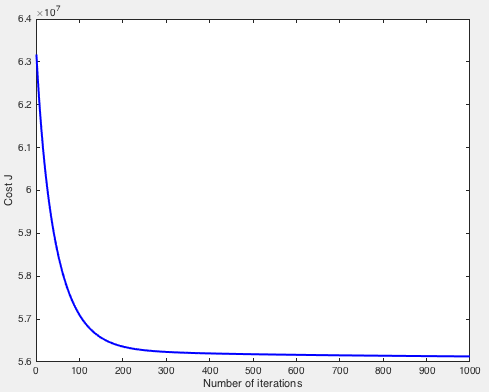
\includegraphics[width=0.4\textwidth]{pics/first_run_001_1000}
	\caption{Cost $J(\theta)$ vs number of iterations graph\label{fig:first_run_label}}   
\end{center} 
\end{figure}   

When the thetas found in the current linearization were applied to the test set, an average error of 3177 shares, and an average percentual error of 169$\%$.

In order to try to improve the errors obtained, a few tweaks were made to the training set. First, elements of higher orders were added to it by taking all features to their 2nd to 12th powers and appending them to the set. This technique may be great to achieve smaller errors within the linear regression using the training set, but it may cause overfitting, which can be tested using the thetas found running the algorithm with the training set with the test set. The cost function graph for this run of gradient descent is shown in Figure ~\ref{fig:second_run_label}.

\begin{figure}[H]
\begin{center}
	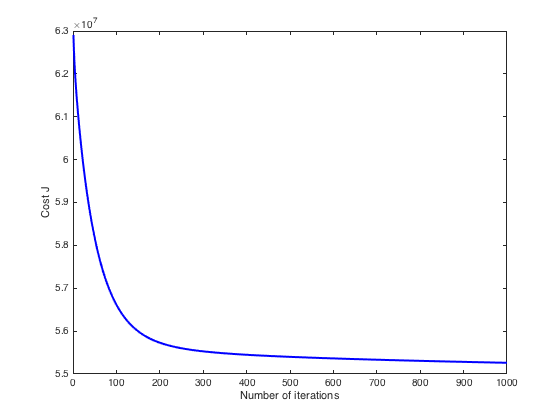
\includegraphics[width=0.4\textwidth]{pics/power_12_wo_reg}
	\caption{Cost $J(\theta)$ vs number of iterations graph with new features of higher order in the training set\label{fig:second_run_label}}
\end{center} 
\end{figure}   

This approach led to a minimal decrease of the errors from the training set, from an average of 3000 shares to 2987 shares. Although that indicator improved, as expected, the error from the test set increased, from an average of 3177 shares to 3204 shares, illustrating an example of slight overfitting. 

In order to try to decrease the effect of overfitting, a regularization method (running gradient descent with the iteration shown in Equation ~\ref{eq:regularization})) was applied to atenuate the higher order weights. Values of $\lambda$ of 1000, 10000 and 100000 were tested, with 100000 giving the smallest error difference between the training and test set, although with a higher training set error compared to not using regularization at all. The average error for the training set was 3020 shares and for the test set, 3190 shares (Figure ~\ref{fig:power_12_with_reg}).

\begin{equation}\label{eq:regularization}
\theta_{j} := \theta_{j}(1 - \alpha \dfrac{\lambda}{m}) - \sum\limits_{i=1}^m  (h_{\theta}(x^{(i)})-y^{(i)})x_{j}^{(i)}
\end{equation}

\begin{figure}[H]
\begin{center}
	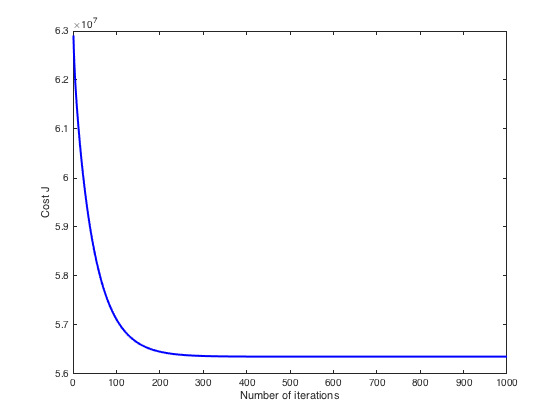
\includegraphics[width=0.4\textwidth]{pics/power_12_with_reg_100k}
	\caption{Cost $J(\theta)$ vs number of iterations graph with new features of higher order in the training set with regularization applied ($\lambda = 100000$)\label{fig:power_12_with_reg}}
\end{center} 
\end{figure}   

Another approach in trying to decrease the prediction error was removing all the discrete variables from the feature set and running gradient descent with the normalized remaining continuous features. As is shown in Figure ~\ref{fig:third_run_label}, the results didn't get better, resulting in an average error of 3021 shares and an average percentual error of 194$\%$. Using the thetas found previously with the features from the test set, an average error of 3195 shares and an average percentual error of 170$\%$ was obtained.

\begin{figure}[H]
\begin{center}
	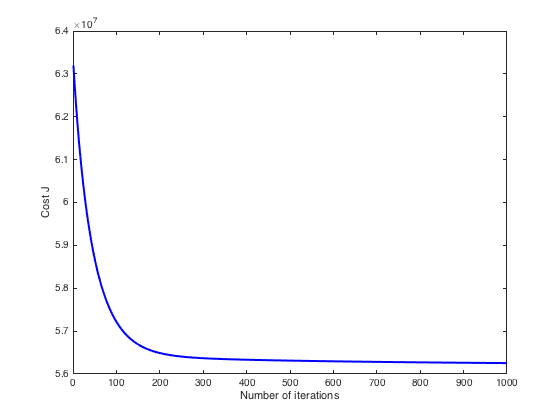
\includegraphics[width=0.4\textwidth]{pics/third_run_001_1000}
	\caption{Cost $J(\theta)$ vs number of iterations graph for training set containing only continuous features\label{fig:third_run_label}}
\end{center} 
\end{figure}   

A great method to find the optimal values of the thetas for a number of features < 5000 is to apply the normal equations method. It consists of a closed formula that utilizes the features matrix $X$ and the target array $y$ and outputs the thetas array $\theta$:

\begin{equation}\label{eq:normal_eq}
\theta = (X^{T}X)^{-1})X^{T}y
\end{equation}

Applying the Equation ~\ref{eq:normal_eq}, and utilizing the result to calculate the errors from the training set, an average error of 2999 shares and an average percentual error of 191$\%$ was obtained. Utilizing the test set, those numbers were 3177 and 165 $\%$, which characterizes a small overfit.

%%% Add section %%%%%%%%%%%%%%%%%%%%%%%%%%%%%%%%%%%%%%%%%%%%%%%%%%%%%%%%%%%%%%%%%%
\section{Discussion}
%%%Talk about the experiments carried out and the obtained results. 

\CITEONE{Silva}{Silva_2010} for papers with one author.
\CITETWO{Silva}{Souza}{Silva_2010b} for papers with two authors.
\CITEN{Silva}{Silva_2010c} for papers with three or more authors.

The standard model for linear regression, when run with a gradient descent algorithm for optimizing the values of theta and with all its features normalized, resulted in a considerably high average error of 3000 shares for the training set and 3177 shares for the test set.

Some modifications were applied to the standard linear regression model in order to find better values of thetas that minimized the cost function. As the features in the training set were taken to higher powers (up to 12th) and added to it, a very small drop in the training set average error (0.4$\%$) was obtained, together with a slight increase in the test set average error (0.9$\%$), showing a glimpse of overfitting. In order to try to mitigate the effects of overfitting, regularization was used, and, with a $\lambda$ = 100000, the difference between the training and test average errors was reduced (3020 and 3190 shares, respectively), but the net error suffered an increase.

When only the continuous features were used, the errors obtained from the training set increased by 0.7$\%$ compared to the initial method and the ones from the test set increased by 0.6$\%$, a very small amount.

By utilizing the normal equations method, which gives an optimal value for the thetas utilizing a pure linearization model, a resulting average training set error of 2999 shares, almost the same as the result found initially (3000 shares) was found.

%%% Add section %%%%%%%%%%%%%%%%%%%%%%%%%%%%%%%%%%%%%%%%%%%%%%%%%%%%%%%%%%%%%%%%%%
\section{Conclusions}

After utilizing various methods and improvements based on linear regression in order to improve the error in the prediction of number of shares, none of them resulted in an acceptable error. 

The minimum average error was 2999 shares for the training set and 3177 shares for the test set utilizing normal equations. A better number was found adding higher order features to the training set (2987 shares), but the distance between its error and the test set one (3204 shares) was higher (overfit). Moreover, trying to reduce the effects of overfitting by using regularization also didn't lead to a better result.

The conclusion that can be taken from the approaches taken is that linear regression is not a good model to represent the problem, and a more complex model must be used in order to account for all the non linearities and intricacies of the dataset.

%%% References %%%%%%%%%%%%%%%%%%%%%%%%%%%%%%%%%%%%%%%%%%%%%%%%%%%%%%%%%%%%%%%%%%%
{\small
\bibliographystyle{unsrt}
\bibliography{referencias-exemplo}
}

\end{document}